\documentclass{article}

% Language setting
% Replace `english' with e.g. `spanish' to change the document language
\usepackage[english]{babel}
% Set page size and margins
% Replace `letterpaper' with `a4paper' for UK/EU standard size
\usepackage[letterpaper,top=2cm,bottom=2cm,left=3cm,right=3cm,marginparwidth=1.75cm]{geometry}
\usepackage{CJKutf8}
% Useful packages
\usepackage{amsmath}
\usepackage{graphicx}
\usepackage{siunitx}
\usepackage[colorlinks=true, allcolors=blue]{hyperref}

\title{Chapter 1: Solving nonlinear equations}
\author{倪爽爽 3210101597\thanks{Email: 3210101597@zju.edu.cn}}


\begin{document}
\begin{CJK}{UTF8}{gbsn}
\maketitle

%\begin{abstract}
%Your abstract.
%\end{abstract}

\section*{A.}

Implement the bisection method, Newton’s method, and the secant method in a C++ package. You should\\
(a) design an abstract base class EquationSolver with a pure virtual method solve,\\
(b) write a derived class of EquationSolver for each method to accomodate its particularities in the con- tract of solving nonlinear equations.\\


\textbf{Answer: }
Construct abstract base class
\begin{verbatim}
    class EquationSolver {
public:
    virtual ~EquationSolver() = default;

    // Solve function that must be overridden in derived classes
    virtual double solve(std::function<double(double)> f, double x0, double x1, double tol) = 0;
};
\end{verbatim}
Construct BisectionSolver, NewtonSolver and SecantSolver respectively according to the algorithm in the book. In NewtonSolver, we design a constructor to accept the derivative function before override solve function from EquationSolver, as Newton method need the derivative function to calculate.



\section*{B.}
Test your implementation of the bisection method on the following functions and intervals.
\begin{itemize}
    \item $x^{-1} - tan x$ on $[0, \frac{\pi}{2} ]$,
    \item $x^{-1} - 2^x$ on $[0, 1]$,
    \item $2^{-x} +e^x +2cosx-6$ on $[1,3]$,
    \item $(x^3 +4x^2 +3x+5)/(2x^3 - 9x^2 +18x - 2)$ on $[0,4]$
\end{itemize}

\textbf{Answer}: 
We design the objective function separately. Taking the \textit{func1} as example, the code is showed below.
\begin{verbatim}
    double func1(double x) {
    return 1.0 / x - tan(x);  // Function: x^{-1} - tan(x)}
    
    double func2(double x) {
    return 1.0 / x - pow(2, x);  // Function: x^{-1} - 2^x}
    
    double func3(double x) {
    return pow(2, -x) + exp(x) + 2 * cos(x) - 6;  // Function: 2^{-x} + e^x + 2*cos(x) - 6}
    
    double func4(double x) {
    return (pow(x, 3) + 4 * pow(x, 2) + 3 * x + 5) / (2 * pow(x, 3) - 9 * pow(x, 2) + 18 * x - 2);  // Function: (x^3 +4x^2 +3x+5)/(2x^3 -9x^2 +18x-2)}
\end{verbatim}
We use the bisection method designed in A.
\begin{verbatim}
    // Test case 1: x^{-1} - tan(x) on [0, π/2]
    double root1 = bisection.solve(func1, 0, M_PI / 2 - 0.1, tol);
    std::cout << "Root for func1: " << root1 << std::endl;
\end{verbatim}
The result of each function will be printed as 
\begin{itemize}
    \item Root for func1: 0.860334
    \item Root for func2: 0.641185
    \item Root for func3: 1.82938
    \item Root for func4: 0.117877
\end{itemize}

\section*{C.}
Test your implementation of Newton’s method by solving x = tan x. Find the roots near 4.5 and 7.7.\\
\textbf{Answer: }\\
We can solve the problem through emunerate shown as below.
\begin{verbatim}
    for (double x0= 45; x0 < 78; x0++)
    {
        double root_C = solver.solve(func_C, x0/10, 0.0, tol);  // x0 = 6.0, tol = 1e-6
    std::cout << "Newton's method result: " << root_C << std::endl;
    };
\end{verbatim}
The result shows that the roots near 4.5 and 7.7 are 4.49341 and 7.72525 respectively.

\section*{D.}
Test your implementation of the secant method by the following functions and initial values.
\begin{itemize}
    \item $sin(\frac{x}{2}) - 1$ with $x_0 = 0, x_1 = \frac{\pi}{2}$,
    \item $e^x-tanx$ with $x_0 =1,x_1 =1.4,$
    \item $x^3-12x^2+3x+1$ with $x_0 =0,x_1 =-0.5.$
\end{itemize}


You should play with other initial values and (if you get different results) think about the reasons.\\


\textbf{Answer: }
In terms of function 1, change the initial values from $x_0 = 0, x_1 = \frac{\pi}{2}$ to $x_0 = \frac{\pi}{2}, x_1 = 4$ as the original result does not lie in $[0,\frac{\pi}{2}]$

The results of function 2 and function 3 is 1.30633 and -0.188685 respectively.

\section*{E.}
As shown below, a trough of length L has a cross section in the shape of a semicircle with radius $r$. When filled to within a distance h of the top, the water has the volume
$$
V=L\left[0.5πr^2 - r^2 arcsin\frac{h}{r} - h(r^2 - h^2)^{\frac{1}{2}}\right]
$$
\begin{figure}[h]
    \centering
    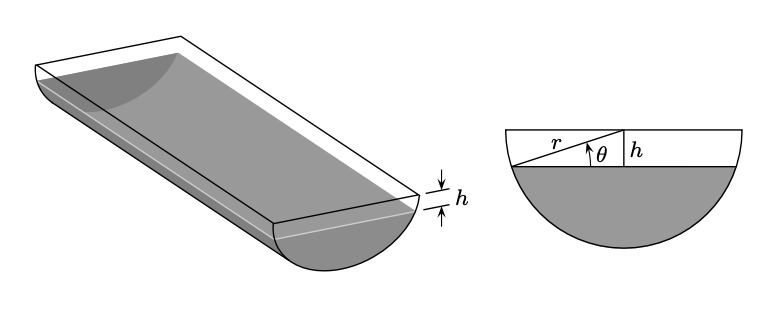
\includegraphics[width=0.5\linewidth]{E.png}
    \caption{Problem E}
    \label{Problem E}
\end{figure}


Suppose $L = 10ft$, $r = 1ft$, and $V = 12.4ft^3$. Find the depth of water in the trough to within 0.01ft by each of the three implementations in A.\\


\textbf{Answer: }

Construct the function and its derivative form as below
\begin{verbatim}
    
double volumeFunction(double h) {  // Function for volume calculation
    double L = 10.0; // length in ft
    double r = 1.0;  // radius in ft
    double targetVolume = 12.4; // desired volume in ft^3
    return L * (0.5 * M_PI * r * r - r * r * asin(h / r) - h * sqrt(r * r - h * h)) - targetVolume;}

double volumeDerivative(double h) {  // Derivative for Newton's method
    double r = 1.0; // radius in ft
    return -10 * ( r+ r * r )/ sqrt(r * r - h * h);}
\end{verbatim}

The result is
\begin{itemize}
    \item Bisection method root (depth of water): 0.166165 ft
    \item Newton's method root (depth of water): 0.166166 ft
    \item Secant method root (depth of water): 0.166166 ft
\end{itemize}

\section*{F.}
In the design of all-terrain vehicles, it is necessary to consider the failure of the vehicle when attempting to negotiate two types of obstacles. One type of failure is called hang-up failure and occurs when the vehicle attempts to cross an obstacle that causes the bottom of the vehicle to touch the ground. The other type of failure is called nose-in failure and occurs when the vehicle descends into a ditch and its nose touches the ground.
\begin{figure}[h]
    \centering
    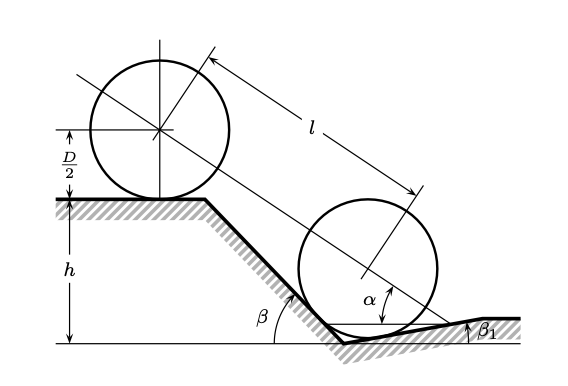
\includegraphics[width=0.5\linewidth]{F.png}
    \caption{Problem F}
\end{figure}


The above figure shows the components associated with the nose-in failure of a vehicle. The maximum angle $\alpha$ that can be negotiated by a vehicle when $\beta$ is the maximum angle at which hang-up failure does not occur satisfies the equation
$$
A sin \alpha cos \alpha + B sin^2 \alpha - C cos \alpha - E sin \alpha = 0,
$$
where 
$$
A = lsin\beta_1, B = lcos\beta_1,
$$
$$
C = (h + 0.5D) sin \beta_1 - 0.5D tan \beta_1,
$$
$$
E = (h + 0.5D) cos \beta_1 - 0.5D.
$$
(a) Use Newton’s method to verify $\alpha \approx 33^{\circ}$ when $l = 89in.$, $h = 49in.$, $D = 55in.$ and $\beta_1 = 11.5^{\circ}$.\\
(b) Use Newton’s method to find $\alpha$ with the initial guess $33^{\circ}$ for the situation when $l$, $h$, $\beta_1$ are the same as in part (a) but $D = 30 in.$.\\
(c) Use the secant method (with another initial value as far away as possible from $33^{\circ}$) to find $\alpha$. Show that you get a different result if the initial value is too far away from $33^{\circ}$; discuss the reasons.\\

\textbf{Answer: }
Change the equations into code,
\begin{verbatim}
    double l = 89;
    double h = 49;
    double beta1 = 11.5 * PI / 180; // convert degrees to radians
    double D1 = 55;
    double D2 = 30;
    double A = l * sin(beta1);
    double B = l * cos(beta1);
    double C1 = (h + 0.5 * D1) * sin(beta1) - 0.5 * D1 * tan(beta1);
    double E1 = (h + 0.5 * D1) * cos(beta1) - 0.5 * D1;
    double C2 = (h + 0.5 * D2) * sin(beta1) - 0.5 * D2 * tan(beta1);
    double E2 = (h + 0.5 * D2) * cos(beta1) - 0.5 * D2;

    auto f1 = [A, B, C1, E1](double alpha) {
        return A * sin(alpha) * cos(alpha) + B * sin(alpha) * sin(alpha) - C1 * cos(alpha) - E1 * sin(alpha);
    };

    auto df1 = [A, B, C1, E1](double alpha) {
        return A * (cos(alpha) * cos(alpha) - sin(alpha) * sin(alpha)) + 2 * B * sin(alpha) * cos(alpha) + C1 * sin(alpha) - E1 * cos(alpha);
    };

    auto f2 = [A, B, C2, E2](double alpha) {
        return A * sin(alpha) * cos(alpha) + B * sin(alpha) * sin(alpha) - C2 * cos(alpha) - E2 * sin(alpha);
    };

    auto df2 = [A, B, C2, E2](double alpha) {
        return A * (cos(alpha) * cos(alpha) - sin(alpha) * sin(alpha)) + 2 * B * sin(alpha) * cos(alpha) + C2 * sin(alpha) - E2 * cos(alpha);
    };
\end{verbatim}
where D1, C1, E1, f1, df1 represent the sub-problem (a) in which $D = 55$, and D2, C2, E2, f2, df2 represent the sub-problem (b) and (c) in which $D = 30$.\\


To solve the problem (a) and (b), load the df1 and df2 respectively and use the \textit{NewtonSolver} to solve.
\begin{verbatim}
    NewtonSolver solver1(df1);
    double alpha1 = solver1.solve(f1, initialGuess, 0.0, tol);
    std::cout << "Alpha for D1 using Newton's method: " << alpha1 * 180 / PI << " degrees" << std::endl;
    
    NewtonSolver solver2(df2);
    double alpha2 = solver2.solve(f2, initialGuess, 0.0, tol);
    std::cout << "Alpha for D2 using Newton's method: " << alpha2 * 180 / PI << " degrees" << std::endl;
\end{verbatim}
To solve the problem (c), we first choose a close point($initialGuess+\frac{PI}{4}$) as the other initial guess. The result is \textbf{33.1689} degrees, same as the result of problem (b) which is solved by newton method.\\


However, if we choose another initial value which is as far away as possible from $33^{\circ}$) to find $\alpha$, 

\begin{verbatim}
    double another_initialGuess = 100;
    double alpha3 = secant.solve(f2, initialGuess, another_initialGuess, tol); // initial guesses far apart
    std::cout << "Alpha for D2 using Secant method: " << alpha3 * 180 / PI << " degrees with " << another_initialGuess << " as another initial Guess" << std::endl;
\end{verbatim}

The result is "Alpha for D2 using Secant method: \textbf{-912567} degrees with 100 as another initial Guess", which deviates greatly from the original correct answer.



\section*{Acknowledgments}
During the preparation of this work the author used ChatGPT to solve the questions and polish the language.

%\bibliographystyle{alpha}
%\bibliography{sample}

\end{CJK}
\end{document}